% Paper draft for FPGA 2013
\pdfminorversion=4
\documentclass[acmtrets]{acmsmall}
\usepackage[binary-units]{siunitx}
\usepackage{algorithm}
\usepackage{algorithmic}
\usepackage[algo2e]{algorithm2e}
\renewcommand{\algorithmcfname}{ALGORITHM}
\SetAlFnt{\small}
\SetAlCapFnt{\small}
\SetAlCapNameFnt{\small}
\SetAlCapHSkip{0pt}
\IncMargin{-\parindent}
\usepackage[flushleft]{threeparttable}
\usepackage[shortlabels]{enumitem}
\usepackage{etoolbox}
\usepackage{bm}
\usepackage{amsmath}
\usepackage[square, comma, sort&compress, numbers]{natbib}
\usepackage[flushleft]{threeparttable}
\usepackage[shortlabels]{enumitem}
\makeatletter
\patchcmd{\maketitle}{\@copyrightspace}{}{}{}
\makeatother

% Metadata Information
\acmVolume{0}
\acmNumber{0}
\acmArticle{1}
\acmYear{2014}
\acmMonth{0}

\usepackage{graphicx}
\usepackage{multirow}
\usepackage[caption=false,font=footnotesize]{subfig}
\usepackage{dblfloatfix}
\usepackage{xspace}
\usepackage{url}

\setlength{\parskip}{0pt}
\renewcommand{\topfraction}{1}
\renewcommand{\textfraction}{0.15}
\renewcommand{\dbltopfraction}{1}

\renewcommand\floatpagefraction{.9}
\renewcommand\topfraction{.9}
\renewcommand\bottomfraction{.9}
\renewcommand\dbltopfraction{.9}
\renewcommand\textfraction{.1}   
\setcounter{totalnumber}{4}
\setcounter{topnumber}{8}
\setcounter{bottomnumber}{4}
\setcounter{dbltopnumber}{4}

\newcommand{\eqnref}[1]{(\ref{#1})}
\newcommand{\figref}[1]{Figure~\ref{#1}}
\newcommand{\algref}[1]{Algorithm~\ref{#1}}
\newcommand{\secref}[1]{Section~\ref{#1}}
\newcommand{\tabref}[1]{Table~\ref{#1}}
\newcommand{\code}[1]{\texttt{#1}}

\newcommand{\tabincell}[2]{\begin{tabular}{@{}#1@{}}#2\end{tabular}}

\graphicspath{{./figures/}}

\begin{document}

\markboth{C.Liu et al.}{An Automatic Nested Loop Acceleration Framework on FPGAs Using Soft CGRA Overlay}
\title{An Automatic Nested Loop Acceleration Framework on FPGAs Using Soft CGRA Overlay}
\author{CHENG LIU
\affil{The University of Hong Kong}
HAYDEN KWOK-HAY SO
\affil{The University of Hong Kong}
}

\begin{abstract}
    The QuickDough design framework is presented as a way to address productivity issues of developing
high-performance FPGA accelerators. QuickDough utilizes a soft coarse-grained reconfigurable array
(SCGRA) as an overlay on top of off-the-shelf FPGAs for rapid accelerator developments.
Instead of compiling high-level applications directly to HDL circuits, the compilation step is
reduced to a simpler operation scheduling task targeting the SCGRA overlay, significantly reducing
compilation time and increasing possible numbers of debug-cycle-per-day as a result.
The softness of the SCGRA allows highly customized application-specific design while the regular
structure of the SCGRA makes the customization much easier. When compared to the
execution on a general purposed processor, the accelerators generated using QuickDough achieves up
to 9X performance speedup.

\end{abstract}

\terms{Nested Loop, FPGA, Overlay, Soft CGRA}
\keywords{Overlay, FPGA Acceleration, Nested Loop, Soft CGRA}

\acmformat{Cheng Liu and Hayden Kwok-Hay So, 2014. 
An Automatic Nested Loop Acceleration Framework on FPGAs Using Soft CGRA Overlay}

\begin{bottomstuff}
This work is supported in part by the Research Grant Concil of Hong
Kong, under the General Research Fund project 716510 and in part by
the Croucher Innovation Award of the Croucher Foundation.

Author's addresses: Cheng Liu and Hayden Kwok-Hay So
Department of Electrical and Electronic Engineering, The University of
Hong Kong, Pokfulam Road, Hong Kong

\end{bottomstuff}

\maketitle

\section{Introduction}
Offloading compute intensive nested loops to FPGA accelerators has 
been demonstrated as an effective way of performance 
acceleration across various application domains\cite{Chung2010}. 
However, the design productivity of developing such accelerators 
remains relatively low and it has become a major obstacle that 
hinders the wide adoption of FPGAs as compute engines. Although the use of 
high level synthesis (HLS) tools which allow the application designers to 
focus on high level functionality instead of low-level implementation details alleviates 
this shortcoming \cite{cong2011high}, the lengthy low-level FPGA implementation process 
greatly limits the number of compile-debug-edit cycles per day and dramatically 
affects the overall design productivity. 

To approach the above design productivity problem, 
researchers have recently turned to the use of virtual FPGA overlay 
architectures \cite{Grant2011Malibu,ZUMA2012,mesh-FUs,
ferreira2011fpga, kissler2006dynamically,scgra}. When combined properly to 
high level compilation tools, the overlay architecture based design methods 
are able to produce high-performance accelerators at near software 
compilation speed, but at the cost of hardware overhead, power and even performance.
By customizing the architectures of these \emph{virtual} 
overlays for a target user design, in theory, it is 
possible to significantly improve the performance-energy of the 
resulting accelerator. In practice, however, navigating through a 
labyrinth of architectural and compilation parameters to fine-tune 
an accelerator's performance-energy is a slow and non-trivial process. 
To require a user to manually explore such vast design space is going 
to counteract the productivity benefit of the utilizing overlay 
in the first place.

To obtain both high design productivity and advantages of 
application-specific customization, we have developed a 
soft CGRA (SCGRA) overlay based nested loop acceleration design 
framework. This framework targets a hybrid CPU-FPGA computing system where 
nested loop compute kernels expressed in high-level languages are compiled and 
executed on the SCGRA overlay built on top of FPGAs while the rest of the 
user application remains running on the host CPU. Given high-level design 
goals and design constraints, the framework automatically explores the 
design space and customizes architectural parameters specifically to the 
user application. In addition, the framework also exploits loop unrolling 
and hardware-software communication strategies in combination 
with buffer sizing and partition as performance enhancing techniques.
Once the design goals and constraints are fulfilled, the 
corresponding hardware accelerator and communication interface 
are generated and both the hardware accelerator and software 
are compiled to the hybrid CPU-FPGA system.  

As demonstrated in previous work, both the compilation from nested 
loops to the SCGRA overlay \cite{scgra} and the SCGRA overlay 
implementation \cite{ROB2014} are fast. Meanwhile, the SCGRA 
overlay is highly pipelined and has quite regular tiling structure, 
which makes the hardware overhead, power consumption and even implementation frequency 
highly predictable. Therefore, a multitude of design metrics such as performance 
and energy consumption can be accurately estimated using analytical models when the 
overlay scheduling result is available. And the nested loop specific acceleration problem can be 
reduced to a sub design space exploration centering an NP-complete SCGRA scheduling and 
a following customization with all the potential configurations well estimated. 
While the overlay scheduling depends on much less design parameters, the overall 
customization can be dramatically simplified. Accordingly, the overall design 
framework achieves both rapid compilation and fast application specific 
customization and ensures high design productivity and high performance of the resulting
accelerators at the same time.  

We performed a series of experiments to evaluate the efficiency 
and quality of the proposed design framework using a real-world 
benchmark. Compared to an exhaustive search, the proposed 
customization achieves similar results while reducing its 
runtime by 2 orders of magnitude on average. When compared to 
HLS implementations with moderate manual optimizations that can 
reasonably be expected from a novice user,  
the customized accelerators produced using the proposed framework 
has demonstrated competitive performance as well. 

With that, we consider the main contribution of this work is in the following areas:
\begin{itemize}[nosep]
\item We have developed a rapid customization framework that 
    performs automatic design parameter tuning for SCGRA overlay based 
    nested loop acceleration on a hybrid CPU-FPGA computing system. 
    The result is comparable to an exhaustive design space search while 
    it runs at a fraction of time.
\item We have developed a parametric regular SCGRA overlay template. It can be used 
    to generate FPGA accelerators with predictable implementation 
    frequency, hardware overhead and power consumption, which is essential to 
    both the rapid compilation and customization.
\item We have developed a hierarchy on-chip buffer. It allows flexible 
    buffer partition and makes good use of the efficient lock-step computation 
    of the SCGRA overlay.
\end{itemize}

In \secref{sec:relatedwork}, related work is briefly introduced. 
The overall automatic nested loop acceleration framework is illustrated 
in \secref{sec:acc-framework}. Then SCGRA overlay based FPGA accelerator 
is illustrated in \secref{sec:scgra} and the application-specific customization 
method is further detailed in \secref{sec:customization-method}. 
Experimental results are presented in \secref{sec:result} and limitations are 
discussed in \secref{sec:limitations}. Finally, the paper is 
concluded in \secref{sec:conclusion}.



\section{Related Work}\label{sec:relatedwork}
Despite their promising performance advantage, the relatively low design productivity of developing
FPGA applications remains a major obstacle that hinders widespread adoption of FPGAs as commodity
computing devices. To address this problem, the design of QuickDough was inspired by the recent success in HLS tools.
It also took advantage of modern FPGAs' capabilities to allow for an additional overlay architecture
be employed for productivity sake.

\subsection{High-Level Synthesis}
To bridge the design productivity gap between software and hardware application development, many researchers have turned to the use of HLS techniques \cite{cong2011high}.
By raising the abstraction level of the physical hardware, HLS allows designers to express hardware designs using familiar high-level, software-like description languages such as C, Java, or Python \cite{cardoso2010compiling,Canis:2011:LHS:1950413.1950423}.
The low-level hardware implementations are then left to the tools to synthesize and optimize.
Indeed, with decades of research, some early results in HLS have already found their ways into FPGA vendors' commercial tools in recent years \cite{chen2005xpilot, zhang2008autopilot, VivadoHLS}.

Unfortunately, when considering the overall design productivity of developing hybrid software-gateware applications, the raised abstraction provided by HLS is only addressing part of the problem.
While the high-level abstraction makes expressing complex functionalities as FPGA gateware easier, the lengthy low-level compilation time spent in synthesis, mapping, placing and routing remains a bottleneck to the overall design productivity for an application designer.
Such long compilation time is particularly challenging for novice designers who are accustomed to the high speed of software compilation.
Most importantly, it is significantly impacting the possible compile-debug-edit cycle achievable per day by a designer, negatively impacting the productivity of the designer.

\subsection{Overlay Architectures}
To improve the speed of low-level implementation tools, researchers have explored various approaches over the past decades.
Inspired by application specific integrated circuit (ASIC) design flows, researchers and vendors have developed modular design flow and explored the use of pre-compiled hard macros \cite{lavin2010using,lavin2011} as implementation library.
In addition, researchers have also exploited the use of dynamic partial reconfiguration capabilities in FPGAs \cite{Frangieh2010} as a way to improve productivity.
In recent years, there has been an increased interest in applying the concept of \emph{overlay architectures} as a way to address this productivity challenge.  


An overlay architecture is a virtual intermediate architecture that is overlaid on top of the physical configurable fabric of an FPGA.  They are employed during the FPGA application implementation process for purposes such as to improve portability, security, and also productivity.
%Depending on the design goal, overlays have manifested in various forms, including HDL models, pre-synthesized or pre-implemented coarse-grained circuits, or even arrays of processing elements with various granularity. 

One of the most familiar categories of overlay consists of virtual FPGAs \cite{zuma2013carl,Grant2011Malibu,Coole2010Intermediate,Koch2013CI}. They are built either virtually or physically on top of off-the-shelf FPGA devices and typically feature coarser configuration granularity than the physical device.
Similar to virtual machines running on a typical computer, such virtual FPGA provides an additional layer that improves application portability and security.
Furthermore, because of the coarser-grained configurable fabric, implementing designs on such overlay is relatively easier than on a fine-grained device.
However, the additional layer imposes restrictions on the underlying fabrics' capability and usually results in moderate hardware overhead and timing degradation.

Another category of overlay architecture commonly employed is in the form of coarse-grained reconfigurable arrays (CGRAs).
The use of CGRAs provides unique advantages of performance especially for compute intensive applications as demonstrated by numerous ASIC CGRAs \cite{tessier2001reconfigurable} \cite{compton2002reconfigurable}.
Indeed, CGRAs on FPGA and ASIC have many similarities in terms of the scheduling algorithm and array structure.
However, they have quite different trade-offs in terms of configuration flexibility, overhead and performance.
In a nutshell, CGRAs on ASIC emphasize more on configuration capability to cover more applications, while FPGAs' inherent programmability greatly alleviates the concern.
Instead, CGRAs on FPGA may take advantage of the configurability of the underlying fabric to allow more intensive customization tailored to the target application.

The authors in \cite{kissler2006dynamically} developed WPPA (weakly programmable processor array), a VLIW architecture based parameterizable CGRA overlay. It featured an interconnection wrapper unit for each processing element (PE) that could be used for dynamic CGRAs topology customization. Unfortunately, programming and compilation on WPPA were not presented. The authors in \cite{ferreira2011fpga} proposed a heterogeneous CGRA overlay with a global multi-stage interconnection on FPGA. Compiling applications onto the overlay took only milliseconds for smaller DFGs. However, the global multi-stage interconnection required multiple stages for communication between each pair of PEs and resulted in either low implementation frequency or large communication latency in terms of cycles. In addition, there was no intermediate storage except the pipeline registers in the CGRA and it limited the performance of the operation scheduling.
In \cite{shukla2006quku}, a customized CGRA overlay called QUKU was developed for DSP algorithms. It had two-level configuration capability, while the low-speed configuration was used for operator reuse within an application and high-speed reconfiguration was used for optimization between different applications. Nevertheless, the hardware infrastructure was consist of simple operation elements which can only be adapted to a few specified DSP algorithms.
The authors in \cite{capalijia2013pipelined} built a more generic high speed mesh CGRA overlay using the elastic pipeline technique to achieve the maximum throughput. It adopted a data-driven execution flow and was suitable for smaller pipelined DFG execution, while it would be difficult to handle applications with random IO access. 

In general, previous CGRA overlays have demonstrated the promising performance acceleration capability for compute intensive applications. They typically take DFG as design entry and focus on hardware infrastructure design as well as corresponding mapping and scheduling. However, they are still lack of consideration on proper loop unrolling for DFG generation, on-chip buffering, the communication with host and even end-to-end performance which are essential for FPGA accelerator design especially from a HW/SW co-design engineer's perspective. 


Finally, a third category of overlay features soft-processor-like architectures with high degree of
control and data parallelism suitable for FPGA accelerations.  For example, in the work of MARC
\cite{Lebedev2010}, a many-core overlay with customizable data path was proposed.  Similarly, a
GPU-like overlay was proposed in \cite{Jeffrey2011potential}.


In this work, we opted to utilize a fully pipelined synchronous soft coarse-grained reconfigurable
array (SCGRA) as an overlay to facilitate rapid FPGA accelerator generation in a hybrid CPU-FPGA
system. Compared to previously proposed CGRAs, our overlay is designed to be \emph{soft} as the size,
processing element designs, as well as the interconnect topologies may all be customized as needed
providing just enough resource for an application specifically. Moreover, the design of our overlay
is regular and design parameters such as loop unrolling factor and overlay size have
relatively predictable influence on the overlay performance and overhead, which makes the
customization much easier and more efficient. Finally, it also takes advantage of the large number
of on-chip distributed memory on the FPGA for intermediate data storage and can handle large DFGs
with thousands of nodes. 

%On top of the above approaches, the use of \emph{overlays} in the form of HDL Model, pre-synthesized or pre-implemented coarse-grained reconfigurable circuits over the fine-grained FPGA devices, promises both to raise the abstraction level and reduce the compilation time.
%Recent years have seen a number of overlay designs being developed with granularities ranging from multi-processors to highly configurable logic arrays \cite{Lebedev2010,kissler2006dynamically,unnikrishnan2009application,Yiannacouras2009FPS,Guy2012VENICE,Jeffrey2011potential}. 

%% Not so much overlay, removed for clarity sake.
%Soft processors, which allow customization for target applications or application domains, have already been demonstrated to be efficient overlays on FPGA. A great number of work use embedded processors as FPGA overlays with micro-architecture parameters such as pipeline depth configurable \cite{Yiannacouras2007Exploration,microblaze,nios} and 


%instruction set architecture (ISA) customizable \cite{grad2009woolcano, }. 


%multi-processor overlay with both micro-architecture and interconnection customizable \cite{unnikrishnan2009application}, 

% vector processors overlay \cite{Guy2012VENICE,Yiannacouras2009FPS}



\section{Automatic Nested Loop Acceleration Framework} \label{sec:acc-framework}
By using a regular SCGRA overlay built on top of the physical FPGA devices, 
we have developed an automatic nested loop acceleration framework targeting 
a hybrid CPU-FPGA system. The goal of the framework is to provide a 
high-productivity nested loop acceleration solution accessible to high-level 
application developers as well as a rapid application-specific 
customization process to achieve better performance-energy trade-off of 
the resulting accelerators. 

\figref{fig:framework} shows the nested loop acceleration framework. Given 
a specified compute intensive loop kernel and high-level design 
goals as well as constraints, the framework automatically 
tunes the design parameters including the SCGRA overlay 
configuration, compilation options and on chip 
communication specifically to the loop kernel through the SCGRA customization 
process. After the customization, corresponding SCGRA overlay based 
FPGA accelerator is generated and implemented through the SCGRA compilation process. 
Meanwhile, the drivers that are needed to utilize the resulting FPGA accelerator 
are generated according to the SCGRA customization. Then the high level application 
is updated and compiled to general purposed processor (GPP) through a 
conventional software compilation process. The application binary code generated in 
combination with the FPGA accelerator bitstream forms the final application 
that will be executed on the hybrid CPU-FPGA system during run time.

\begin{figure}[tb]
\center{\includegraphics[width=0.75\linewidth]{framework}}
\caption{Automatic nested loop acceleration framework}
\label{fig:framework}
\end{figure} 

SCGRA customization process is the focus of this work where optimal 
design choices are decided. Since it involves exploration in a vast 
design space, it is critical to the design productivity of the whole 
framework. In addition, it also determines the configurations of 
the resulting accelerators and thus affects the performance-energy 
trade-off of the final design. In this work, a dedicated customization 
method is proposed to meet both the requirements of the design productivity and 
performance-energy trade-off and it will be further illustrated in the following 
sections.

SCGRA compilation is responsible for mapping the high-level loop 
kernel to the physical FPGA bitstream through a specified SCGRA 
overlay. \figref{fig:horizontal-compilation} presents an overview of the 
compilation process and it includes two compilation flows for two typical
development scenarios i.e. initial compilation and iterated compilation. 
In the first scenario when the specified SCGRA overlay is initially 
implemented on the target physical FPGA device, a standard implementation 
from HDL model may be time-consuming. Fortunately, a hardware-macro compilation 
technique \cite{ROB2014} developed for the regular tiling architectures may 
significantly decrease the implementation time. In the second scenario when 
the specified SCGRA overlay has already been implemented, the bitstream can 
be reused as demonstrated in \cite{scgra} and the compilation can be reduced to seconds.

\begin{figure}[tb]
\center{\includegraphics[width=0.8\linewidth]{horizontal-compilation}}
\caption{High-productivity SCGRA overlay compilation, The whole diagram represents the initial
compilation and it includes both the iterated compilation and the initial implementation.}
\label{fig:horizontal-compilation}
\end{figure}



\section{SCGRA overlay based FPGA acceleration} \label{sec:scgra}
In this work, parametric and scalable SCGRA overlay architectures, 
on-chip buffer structures and loop execution strategies 
have been developed for the nested loop acceleration framework. These 
design choices provide unique opportunity for application specific customization 
and help to achieve better performance-energy trade-off of the resulting accelerators.

\subsection{SCGRA Overlay Based FPGA Accelerator}
\figref{fig:scgra-acc} shows the design of a typical SCGRA overlay 
based FPGA accelerator. In the accelerator, on-chip
memory i.e. IBuf and OBuf are used to buffer the communication 
data between the host CPU and the accelerator. A controller is also 
presented in hardware to control the operations of the accelerator as well as
memory transfers. The SCGRA, which is the kernel computation fabric,
consists of an array of processing elements (PEs) and it achieves the computation 
task through the distributed control words stored in each PE. 

PE is the key design element of the SCGRA overlay. It is simple yet 
highly pipelined which is beneficial to the hardware implementation. At the 
heart of PE is an ALU, which is supported by a multi-port data memory and 
an instruction memory. Three of the data memory's read ports are connected 
to the ALU as inputs, while the remaining ports are sent to the output 
multipliers for connection to neighboring PEs and the optional store paths 
external to the SCGRA overlay. At the same time, this data memory takes input 
from the ALU output, data arriving from neighboring PEs as well as from the 
optional IBuf loading path. The action of the PE is controlled by the AccCtrl unit 
that reads from the instruction memory. Finally a global signal from the AccCtrl 
block controls the start/stop of all PEs in the array.

ALU carries out the computations of the given applications. It can be easily customized 
to support operations of a specified application or a group of applications. The supported
operations are fully pipelined in the ALU and may execute concurrently while they must 
complete in a deterministic number of cycles. Since ALU has only a single output port, 
the scheduler will ensure that there is never conflict at the output.
\begin{figure}[tb]
\center{\includegraphics[width=0.99\linewidth]{scgra-accelerator}}
\caption{SCGRA overlay based FPGA accelerator}
\label{fig:scgra-acc}
\end{figure}

\subsection{Loop execution on the accelerator}
\figref{fig:group-dfg} illustrates how the loop is executed 
on the FPGA accelerator. First of all, data flow graph (DFG) is extracted 
from the loop and then it is scheduled on to the SCGRA overlay based FPGA accelerator. 
Depending on how much the loop is unrolled and transformed to DFG, the DFG may be 
executed repeatedly until the end of the original loop. In addition, data transfers for 
multiple executions of the same DFG are batched into groups as shown in \figref{fig:group-dfg}. 
On the one hand, this technique is used to reduce the number of batching, which further 
helps to amortize the initial communication cost. On the other hand, it also 
results in larger on-chip memory overhead. The proposed customization framework 
can be used to make the right design choices to achieve an optimal design. 

\begin{figure}[tb]
\center{\includegraphics[width=0.95\linewidth]{group-dfg}}
\caption{Loop, group and DFG. The loop will be divided into 
groups. Each group will be partially unrolled and the unrolled part will be 
translated to DFG. IO transmission between FPGA and host CPU is performed 
in the granularity of a group.}
\label{fig:group-dfg}
\end{figure}

\subsection{On-chip buffer structure}
On-chip buffer is used to store data transmitted between the FPGA 
accelerator and main memory. (The input and output buffers are quite similar, so 
we just present the input buffer structure here for saving the space.) 
It is usually implemented with block RAM and 
a naive implementation as shown in \figref{fig:naive-implementation} 
provides limited bandwidth to the accelerator which may dramatically 
restrict the performance of the accelerator. A straightforward solution is to 
expose the primitive block RAM ports to the accelerator 
directly as shown in \figref{fig:quick-partition}. However, the bandwidth is 
limited by the number of the primitive block RAM and it works only when 
the data is perfectly placed into different block RAM banks and each port of 
the accelerator accesses exactly the corresponding sub set of the data. In addition, 
we may want to have the input/output data of the same group stored in the input/output 
buffers as mentioned in previous section, while different input/output of the 
DFGs in the same group may have diverse layout pattern. For instance, one DFG 
may load its first input data from partitioned bank 0 while the 
following DFG may have to load its first input data from bank 1. As a result, 
the two DFGs will not be able to reuse the same lock-step computing on the SCGRA overlay. 
Although we may load/store input/output data for each DFG computation, the 
fine-grain data transmission between main memory and FPGA on-chip buffer is extremely 
expensive.

To solve this problem, we have introduced an additional buffering stage and developed 
a scalable on-chip buffer structure as shown in \figref{fig:scalable-partition1} 
and \figref{fig:scalable-partition2}. The first stage is the basic on-chip buffer as 
mentioned in \figref{fig:naive-implementation} and \figref{fig:quick-partition}. It stores 
data of a single transmission between the accelerator and main memory. The additional 
buffer stage stores the input/output of the DFG computation on the CGRA overlay. It ensures the 
input/output data has exactly the same layout for all the DFG computation. Moreover, it can be 
implemented with arbitrary number of FIFOs providing sufficient bandwidth to the accelerator. 

\begin{figure}[tb]
    \centering
	\subfloat[Naive buffer structure]{%
		\includegraphics[width=0.3\textwidth]{buffer-type0}
        \label{fig:naive-implementation}
	}\qquad
	\subfloat[Straightforward partitioned buffer structure]{%
		\includegraphics[width=0.35\textwidth]{buffer-type1}
        \label{fig:quick-partition}
	}
    \hfill
	\subfloat[Naive partitioned buffer structure]{%
		\includegraphics[width=0.45\textwidth]{buffer-type2}
        \label{fig:scalable-partition1}
	}
	\subfloat[Scalable partitioned buffer structure]{%
		\includegraphics[width=0.55\textwidth]{buffer-type3}
        \label{fig:scalable-partition2}
	}
    \caption{On-chip buffer structure}
	\label{fig:on-chip-buffer}
\end{figure}


Although the additional buffer stage makes the computation data path even 
longer, data movement between the first buffer stage and the second buffer 
stage in input/output buffer and the DFG computing in the same group can 
be pipelined as illustrated in \figref{fig:buffer-pipelining}. 
As long as the FIFOs are still available, FlowCtrl will keep the 
first stage buffer sending data to the second buffer stage with the 
pre-scheduled order which is obtained from the CGRA overlay scheduling 
and stored in the AddrBuffer. When the FIFOs have all the input for a 
single DFG execution, FlowCtrl will start the accelerator. When the 
accelerator completes a DFG computing, it will stop until it is activated 
next time. On the output side, the buffer and the accelerator work similarly.
When the number of DFGs included in a group is big enough and DFG computing 
time is larger than the data movement cost, the cost of the 
additional buffer stages can be ignored. 

To support the pipelining in \figref{fig:buffer-pipelining}, 
the overall FIFO capacity is set to be twice the input/output 
of a single DFG. When the time consumed for data movement between 
the two buffer stages is shorter than the DFG computing time, 
\figref{fig:scalable-partition1} can be used. Or else, we may 
make use of all the potential bandwidth in the first buffer stage using 
the buffer in \figref{fig:scalable-partition2}. 

\begin{figure}[tb]
\center{\includegraphics[width=0.9\linewidth]{buffer-pipelining}}
\caption{Pipelined execution on the CGRA overlay}
\label{fig:buffer-pipelining}
\end{figure}



\section{SCGRA Overlay Based FPGA Accelerator Customization} \label{sec:customization-method}
Application-specific customization provides unique opportunity to improve 
the power-performance of the resulting accelerators. However, 
taking the system as a black box and exhaustively searching all the 
possible configurations may be inefficient and slow, which will 
result in low design productivity. In this work, by taking advantage 
of the regularity of the SCGRA overlay based FPGA accelerator, we 
can reduce the complex customization problem to a small DSE together with 
a simplified customization problem, and near optimal application-specific 
nested loop acceleration can be achieved rapidly.

\subsection{Customization Framework}
\figref{fig:customization-framework} illustrates the overview of the 
customization framework. It can be roughly divided into two 
parts. In the first part, a sub DSE targeting loop execution time 
is performed and the feasible design space can be acquired. Since loop 
execution time is determined by the operation scheduling 
which merely depends on the loop unrolling factor and SCGRA size, the 
sub DSE is much simpler compared to the overall system DSE. 

In the second part, each configuration 
in the feasible design space will be evaluated. Instead of using simulation 
based methods, analytical models are employed to estimate the accelerator 
metrics such as performance, overhead, energy consumption etc.. 
Because of the regularity of the SCGRA overlay, these analytical models are accurate. 
Even though the feasible design space is still large, it is fast to evaluate 
all the configurations in the feasible design space. After the evaluation process, 
customization for various design goals becomes trivial and the customized 
design parameters can be obtained immediately.

\begin{figure}[t]
\center{\includegraphics[width=0.55\linewidth]{customization-framework}}
\caption{System customization framework.}
\label{fig:customization-framework}
\end{figure}

\subsection{Customization Problem Formulation}
In this section, we will formalize the customization problem 
of the nested loop acceleration on an SCGRA overlay based FPGA accelerator. 
Various design goals including performance, energy consumption and 
energy delay product (EDP) are used while energy consumption is taken 
as an example here.
\begin{table}
  \tbl{Design Parameters of Nested Loop Acceleration\label{tab:parameter-list}}{
  \centering
  \tiny
  \resizebox{0.8\columnwidth}{!}{
      \begin{tabular}{l|l|l}
          \hline
          \multicolumn{2}{l|}{Design Parameters} & Denotation \\ \hline
          \multirow{2}{*}{\tabincell{l}{Nested Loop \\ Compilation}} & Loop Unrolling Factor & $\bm{u}=(u_0,u_1, ...)$  \\ \cline{2-3} 
                                                                     & Grouping Factor & $\bm{g}=(g_0, g_1, ...)$ \\ \hline
          \multirow{11}{*}{\tabincell{l}{Overlay \\ Configuration}}  & SCGRA Topology  & Null, 2D Torus \\ \cline{2-3} 
                                                                     & SCGRA Size  & $r\times c$ \\ \cline{2-3}
                                                                     & Instruction Mem & $imD \times imW$ \\ \cline{2-3}
                                                                     & Data Mem & $dmD \times dmW$ \\ \cline{2-3}
                                                                     & Input Buffer & $ibD \times ibW$ \\ \cline{2-3}
                                                                     & Output Buffer & $obD \times obW$ \\ \cline{2-3}
                                                          & Input Address Buffer & $iabD \times iabW$ \\ \cline{2-3}
                                                          & Output Address Buffer & $oabD \times oabW$ \\ \cline{2-3}
                                                          & Operation Set & Null, fixed \\ \cline{2-3}
                                                          & Implementation Frequency & $f$, fixed \\ \hline
                                                          & Pipeline Depth & Null, fixed \\ \hline
\end{tabular}
 
  }
  }
\end{table}


Suppose $\bm{\Psi}$ represents the overall nested loop acceleration design 
space. $\bm{C} \in \bm{\Psi}$ represents a possible configuration in 
the design space and it includes a number of design parameters as  
listed in \tabref{tab:parameter-list}. Assume that the loop to be accelerated 
has $n$ nested levels and loop count can be denoted as $l=(l_1, l_2, ..., l_n)$.
$R=(R_1, R_2, R_3, R_4)$ stands for the FPGA resource (i.e. BRAM, DSP, LUT and FF) 
that are available on a target FPGA and $Overhead(\bm{C}, i)$ denotes the 
four different types of FPGA resource overhead. $In(\bm{g})$ and $Out(\bm{g})$ 
stand for the amount of input and output of a group. Similarly, $In(\bm{u})$ 
and $Out(\bm{u})$ stand for the amount of input and output of a DFG. 
$DFGCompuTime(\bm{C})$ represents the number of cycles needed to 
complete the DFG computation. $\alpha_i$ and $\beta_i$ are constant 
coefficients depending on target platform where $i=(1,2,...)$. With these denotations, 
the customization problem targeting minimum energy consumption can be formulated 
as follows:

Minimize 
\begin{equation} \label{eq:energy}
    Energy(\bm{C})=Power(\bm{C}) \times (\frac{RunTime(\bm{C})}{f})
\end{equation}
subject to
\begin{equation} \label{eq:constraints}
    \begin{split}
        &Overhead(\bm{C}, i) \leq R_i, i=1,2,3,4 \\
        &In(g) \leq ibD \\
        &Out(g) \leq obD \\
        &DFGCompuTime(\bm{C}) \leq imD \\
        &\displaystyle \prod_{i=1}^{n} \frac{g_i}{u_i} \times In(u) \leq iabD \\
        &\displaystyle \prod_{i=1}^{n} \frac{g_i}{u_i} \times Out(u) \leq oabD
    \end{split}
\end{equation}

$RunTime(\bm{C})$ represents the number of cycles needed to compute the loop on 
the CPU-FPGA system. It consists of both the time consumed for computing on FPGA and 
communication between FPGA and host CPU, and it can be calculated using \eqnref{eq:runtime}.

\begin{equation} \label{eq:runtime}
    RunTime(\bm{C})=CompuTime(\bm{C})+CommuTime(\bm{C})
\end{equation}

Since the unrolled part of the loop will be translated to 
DFG and then scheduled to the SCGRA overlay. Thus the DFG computation time 
is essentially a function of $\mathbf{u}$, $r$ and $c$, and it can also be 
denoted by $DFGCompuTime(\mathbf{u},r,c)$.
The nested loop is computed by repeating the same DFG execution, and the 
nested loop computation can be calculated using \eqnref{eq:loopexetime}.
\begin{equation} \label{eq:loopexetime}
    CompuTime(\bm{C})=\displaystyle \prod_{i=1}^{n} \frac{l_i}{u_i} \times DFGCompuTime(\mathbf{u},r,c)
\end{equation}

DMA is typically used for the bulk data transmission. Communication cost per 
data can be modeled with a piecewise linear function and thus DMA latency can be 
calculated using \eqnref{eq:DMA}.

\begin{equation} \label{eq:DMA}
    DMA(x)=%
    \begin{cases}
        (\alpha_1\times x + \beta_1) \times x &: (x \leq T_0) \\
        (\alpha_5\times x + \beta_5) \times x &: (T_0 < x \leq T_1) \\
        \alpha_6\times x &: (x > T_1)
    \end{cases}
\end{equation}

where $x$ represents the amount of DMA transmission and $T_0, T_1$ stand for 
the turning points of the piecewise function. The communication time of the 
whole nested loop can be calculated by \eqnref{eq:commu}.
\begin{equation} \label{eq:commu}
    CommuTime(\bm{C})=\displaystyle \prod_{i=1}^{n} \frac{l_i}{g_i} \times 
    (DMA(In(\mathbf{g}))+DMA(Out(\mathbf{g})))
\end{equation}

Power consumption of the FPGA accelerator consists of 
BRAM power, clock power, signal power and so on. 
Various experiments were done to measure the BRAM power and 
we can model BRAM power as \eqnref{eq:brampower}. 
The rest part of the hardware resource mainly changes with the SCGRA size, 
so the power consumption can be roughly modeled with a linear 
equation of SCGRA size. Therefore, the power consumption 
of the accelerator can be modeled by \eqnref{eq:totalpower}.
\begin{equation} \label{eq:brampower}
    Power\_BRAM(\bm{C})=\alpha_7 \times r \times c \times Overhead(\bm{C}, 1)
\end{equation}

\begin{equation} \label{eq:totalpower}
    Power(\bm{C})=Power\_BRAM(\bm{C})+\alpha_8 \times r \times c + \beta_6
\end{equation}

Hardware overhead on FPGA mainly includes DSP, LUT, FF and 
BRAM (block RAM). LUT, FF and DSP overhead can be roughly estimated 
with a linear function of SCGRA size and can be calculated using \eqnref{eq:dsplutff}. 
BRAM overhead which is usually the overhead bottleneck for SCGRA overlay based 
FPGA accelerator design can be calculated by \eqnref{eq:bramoverhead}.
\begin{equation} \label{eq:dsplutff}
    Overhead(\bm{C}, i)=\alpha_i \times r \times c + \beta_i, (i=2,3,4)
\end{equation}
\begin{equation} \label{eq:bramoverhead}
    \begin{split}
        Overhead(\bm{C}, 1)=&r \times c \times (imD \times imW + dmD \times dmW) + \\
                               &(ibD \times ibW + obD \times obW) + (iabD \times iabW + oabD \times oabW) 
    \end{split}
\end{equation}

\subsection{Proposed Customization Method}
Almost all the design metrics can be estimated by the analytical models when 
the operation scheduling result is available. Since the scheduling result 
merely depends on unrolling factor and the SCGRA overlay size, we can separate 
the scheduling from the customization problem and perform a sub DSE to 
reduce the large design space to a smaller feasible design space. Within 
the feasible design space, we further search the optimized design parameter 
for the entire system customization.

Suppose $\Phi$ denotes the feasible design space. $\epsilon$ indicates the
percentage of the performance benefit obtained by the increase 
of loop unrolling or SCGRA size. It is a user defined 
threshold and must be small enough to prune the configurations that are 
inappropriate. The configurations in $\Phi$ must satisfy \eqnref{eq:cond1} 
and \eqnref{eq:cond2}. 
\begin{equation} \label{eq:cond1}
    \begin{split}
        &\forall \bm{C}=(...,\bm{u},r,c,...)\in \Phi, \bm{C'}=(...,\bm{u'},r',c',...) \in
        \Phi,(r+1==r' \text{ and } c==c') \text{ or } \\ 
        &(r==r' \text{ and } c+1==c'): \\ 
        &\frac{CompuTime(\bm{C})-CompuTime(\bm{C'})}{CompuTime(\bm{C})} > \epsilon \\
    \end{split}
\end{equation}

\begin{equation} \label{eq:cond2}
    \begin{split}
        &\forall \bm{C}=(...,\bm{u},r,c,...) \in \Phi, \bm{C'}=(...,\bm{u'},r,c,...) \in \Phi, \bm{u} \text{ and } \bm{u'} \text{ are consecutive unrolling factors}: \\
        &\frac{CompuTime(\bm{C})-CompuTime(\bm{C'})}{CompuTime(\bm{C})} > \epsilon
    \end{split}
\end{equation}

Each configuration $\bm{C} \in \Phi$ must have the corresponding 
scheduling result known, and thus the computation time of the 
loop kernel, minimum instruction memory depth and data buffer 
depth are available as well. Then we can further evaluate 
energy consumption of each feasible configuration using the models built in 
previous section and acquire the optimized configuration.

In order to achieve the desired customization, we must make sure the 
feasible design space acquired from \eqnref{eq:cond1} and \eqnref{eq:cond2} can always 
cover the configuration that produces the optimal customization. A brief 
proof is presented as follows.

$\forall \bm{C'} \notin \Phi$, there must be a configuration $\bm{C}$ that fails 
\eqnref{eq:cond1} or \eqnref{eq:cond2}. Suppose $\bm{C'}=(...,\bm{u},r+1,c,...)$ 
and $\bm{C}=(...,\bm{u},r,c,)$. Thus we can conclude that 
\begin{equation}
    CompuTime(\bm{C'}) \geq (1-\epsilon) \times CompuTime(\bm{C})
\end{equation}

Since $\epsilon$ can be small and unrolling factor is not changed, $DFGCompuTime(\bm{C'})$ 
roughly equals to $DFGCompuTime(\bm{C})$ and therefore the instruction memory depth 
will not change. However, the increase of row size of the SCGRA overlay will result in 
significant overhead of BRAM and power consumption. Thus $Power(\bm{C'}) 
\geq Power(\bm{C})$. In addition, it will reduce the BRAM budget 
for on-chip buffer, which means $CommuTime(\bm{C'}) \geq CommuTime(\bm{C})$. 
According to \eqnref{eq:energy} and \eqnref{eq:runtime}, it is clear 
that $Energy(\bm{C'}) \geq Energy(\bm{C})$ and 
any configuration that is pruned during the sub DSE will not be an optimized 
configuration. Similarly, we can also draw the same conclusion when a different 
occasion in \eqnref{eq:cond1} and \eqnref{eq:cond2} appears.

In addition, a series of experiments on Zedboard \cite{zedboard} as 
shown in \figref{fig:observation} demonstrate that SCGRA size and 
unrolling factor present a clear monotonic influence on the 
loop compute time. The performance benefit of loop unrolling and 
increase of SCGRA size drops gradually and thus we can conclude that \eqnref{eq:observation}.
\begin{equation} \label{eq:observation}
    CompuTime(\bm{C_1})-CompuTime(\bm{C_2}) > CompuTime(\bm{C_2})-CompuTime(\bm{C_3})
\end{equation}
where $\bm{C_1}=(...,x1,...)$, $\bm{C_2}=(...,x2,...)$, $\bm{C_3}=(...,x3,...)$ and
$x1$, $x2$, $x3$ are three increasingly consecutive configurations of loop unrolling 
factor or row or column of the SCGRA overlay.

In other words, if $\bm{C_1}$ fails to be a feasible configuration, we can be 
sure that $\bm{C_2}$ and $\bm{C_3}$ will fail as well. With this observation, 
we can further simplify the sub design space exploration. The simplified sub 
DSE will be detailed in next section.

\begin{figure}[tb]
    \centering
    \subfloat[\label{fig:scgrasize-perf}]{%
      \includegraphics[width=0.3\textwidth]{scgrasize-perf}
    }
    \qquad
    \subfloat[\label{fig:unrolling-perf}]{%
      \includegraphics[width=0.3\textwidth]{unrolling-perf}
    }
    \caption{The design parameters typically have monotonic influence on the
        loop computation time and the computation time benefit degrades with 
        the increase of the design parameter. (a) SCGRA Size, (b) Unrolling Factor}
    \label{fig:observation}
  \end{figure}


\subsection{Sub Design Space Exploration}
To acquire the feasible design space, we developed a dedicated sub DSE 
targeting nested loop computation time. Since the loop computation 
time merely depends on the SCGRA overlay 
size and the loop unrolling factor, the sub DSE is much simpler 
compared to the overall customization problem. In addition, we can 
further simplify the sub DSE with the observations shown in \figref{fig:observation}.  
Whenever a configuration fails the sub DSE condition, all the 
configurations which are larger on one design parameter and remain the same 
on the rest design parameters can be safely pruned. Thus a branch and 
bound algorithm as detailed in \algref{alg:revenuealg} is used 
to efficiently explore the sub design space.
\begin{algorithm}[h]
\caption{Sub Design Space Exploration.}
\label{alg:revenuealg}
\begin{algorithmic}
\PROCEDURE{}
\STATE Initialize $r=2, c=2, \bm{u}=(1,1,...)$, feasible design space $\Phi=\emptyset$,
$\bm{C}=(...,r,c,\bm{u},...)$, maximum SCGRA overlay $r_{Max}\times c_{Max}$.
\WHILE {$r<r_{Max}$} 
\WHILE {$c<c_{Max}$}
\WHILE {$\bm{u}$ is not fully unrolled}
\STATE Generate DFG with $\bm{u}$
\STATE DFG Scheduling with configuration $\bm{C}$
\STATE Estimate performance $CompuTime(\bm{C})$
\STATE Get neighbor $\bm{C'} \in \Phi$ with smaller loop unrolling
\IF {$\bm{C'}$ exists and $Revenue(\bm{C}, \bm{C'}) \leq \epsilon$}
\STATE Break
\ELSE 
\STATE Add $\bm{C}$ to $\Phi$
\ENDIF
\STATE update $\bm{u}$ with larger neighbor unrolling factor
\ENDWHILE
\STATE Get neighbor $\bm{C''} \in \Phi$ with smaller column size
\IF {$\bm{C''}$ exists and $Revenue(\bm{C}, \bm{C''}) \leq \epsilon$}
\STATE Break
\ENDIF
\STATE $c=c+1$
\ENDWHILE
\STATE Get neighbor $\bm{C'''} \in \Phi$ with smaller row size
\IF {$\bm{C'''}$ exists and $Revenue(\bm{C}, \bm{C'''}) \leq \epsilon$}
\STATE Break
\ENDIF
\STATE $r=r+1$
\ENDWHILE
\ENDPROCEDURE
\STATE
\PROCEDURE {$Revenue(\bm{C}, \bm{C'})$}
\STATE return $\frac{CompuTime(\bm{C'})-CompuTime(\bm{C})}{CompuTime(\bm{C'})}$ 
\ENDPROCEDURE
\end{algorithmic}
\end{algorithm}



\section{Experiments and results} \label{sec:result}

\subsection{Experiment Setup}
environment and benchmark applications

\subsection{Performance on Different Memory Models}

\subsection{Simulation Speed and Precision}


\section{Conclusion} \label{sec:Conclusion}
In this paper, we propose to take the CNN accelerator’s ‘undeterministic’ behaviors into consideration 
at training and have the CNN model to learn the accelerator’s behaviors. To that end, we further build 
an open-sourced training system based on Caffe on a hybrid CPU-FPGA architecture. Then use the training 
system to deal with an overclocked CNN accelerator and an accelerator with soft errors. According to our 
experiments, the proposed training can improve the prediction accuracy of four CNN models up to 3.4\% when 
the CNN accelerator is overclocked on the extreme situation. This method is also beneficial to the CNN 
accelerators with soft errors. In the case with most soft errors, it improves the prediction accuracy up 
to 6.8\% and by 3.58\% on average. The disadvantage is the much longer training time due to the frequent 
data transfer between host memory and device memory. This problem can be resolved when porting the system 
to closely coupled CPU-FPGA architectures with shared memory.

%\appendix
%\section{Acknowledgement}

%\begin{acks}
%  The authors would like to thank Sam Ho for providing the suggestions on
%  HLS design debugging and optimization as well as the SDAccel usage. 

%\end{acks}


\bibliographystyle{newapa}
{\small\bibliography{refs}}

%\balancecolumns
\end{document}

